\documentclass[aspectratio=1610]{beamer}

\usepackage{graphicx}
\usepackage[english]{babel}
\usepackage[T1]{fontenc}
\usepackage{csquotes, xcolor, xspace, changepage, setspace, listings}
\usepackage{libertinus}
\usepackage{roboto}
\usepackage{fontawesome5}
\usepackage[scale = 0.75]{plex-mono}
\usepackage{tikz, subcaption}

\usetikzlibrary{fit, shapes.geometric, shapes.symbols, positioning, shapes.misc, calc, arrows.meta, patterns, backgrounds, decorations, decorations.markings, decorations.pathreplacing, shadows, hobby}

\usepackage[backend=bibtex,style=authoryear]{biblatex}
\addbibresource{biblio.bib}

\title{Human Pose Estimation}
\author{Roland Bernard}
\date{February 2026}

\definecolor{unibzblue}{HTML}{0086ec}
\definecolor{unibzblue2}{HTML}{f0f8ff}

\setbeamercolor{outerbox}{fg=black,bg=unibzblue2}
\setbeamercolor{innerbox}{fg=white,bg=unibzblue}

\setbeamertemplate{title page}{
  \scriptsize 
  \begin{tabular}{ll}
    \vspace*{40mm} \\
    \multicolumn{2}{l}{\raggedright Progress Update -- Capstone Project 2025/2026} \\
    \\
    \multicolumn{2}{p{\linewidth}}{\raggedright \huge \bf \inserttitle} \\
    \\
    \\
    & \insertauthor \\
    \\
    & \insertdate \\
  \end{tabular}
}

\setbeamertemplate{frametitle}{
  \vspace*{6mm}
  \Large \bf \color{black} \insertframetitle
}

\setbeamertemplate{itemize items}{\scriptsize\raisebox{0.6mm}{\color{unibzblue} $\blacktriangleright$}}

\beamertemplatenavigationsymbolsempty
\setbeamertemplate{footline}{
  \begin{beamercolorbox}[wd=\paperwidth,right]{section in head/foot}
    \usebeamerfont{date in head/foot}\hspace*{2em}
    \insertframenumber{}\hspace*{2mm} 
    \vspace*{2mm}
  \end{beamercolorbox}
}

\newcommand{\litem}{{\scriptsize\raisebox{0.6mm}{\color{unibzblue} $\blacktriangleright$}}}
\newcommand{\sitem}{{\scriptsize\raisebox{0.2mm}{\color{unibzblue} $\rightarrow$}}\enspace}
\newcommand{\icon}[1]{\textcolor{unibzblue}{\faIcon[solid]{#1}}}

\newlength{\offsetpage}
\newenvironment{narrowpage}[1][3mm]{
  \setlength{\offsetpage}{#1}
  \begin{adjustwidth}{\offsetpage}{\offsetpage}
}{
  \end{adjustwidth}
}
\newenvironment{widepage}[1][10mm]{
  \setlength{\offsetpage}{#1}
  \begin{adjustwidth}{-\offsetpage}{-\offsetpage}
}{
  \end{adjustwidth}
}

\newenvironment{items}{
  \begin{narrowpage}
}{
  \end{narrowpage}
}
\newenvironment{oitem}[2][3mm]{
  \vspace*{2mm}
  \begin{beamercolorbox}[rounded=false,colsep=#1]{outerbox}
    \parbox[t]{2mm}{\centering#2}\parbox[t]{2mm}{\ }%
    \begin{minipage}[t]{\linewidth}
}{
    \end{minipage}
  \end{beamercolorbox}
  \vfill
}

\begin{document}

\begin{frame}[plain]
  \begin{tikzpicture}[
    remember picture, overlay,
    every path/.style={opacity=0.10},
    yshift=20, xshift=200, scale=1.5, transform shape
  ]
    \node {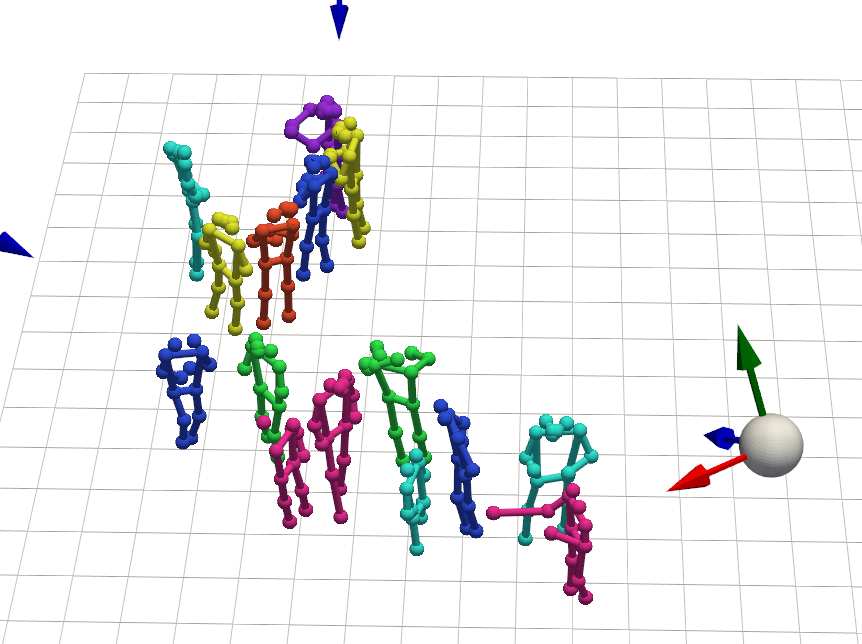
\includegraphics[width=0.9\linewidth]{figures/background.png}};
  \end{tikzpicture}
  \titlepage
\end{frame}

\begin{frame}
\frametitle{Task -- Human Pose Estimation}
  \begin{items}
    \begin{oitem}{\litem}
      Given: \\
      \sitem {\footnotesize Multiple video sequences containing multiple people.} \\
      \sitem {\footnotesize Recorded using multiple calibrated cameras.}
    \end{oitem}
    \begin{oitem}{\litem}
      Reconstruct: \\
      \sitem {\footnotesize 3D coordinates of skeletal joint for each subject.} \\
      \sitem {\footnotesize Movement of skeletal joint over time.}
    \end{oitem}
    \vspace*{2mm}
    \begin{figure}
      \centering
      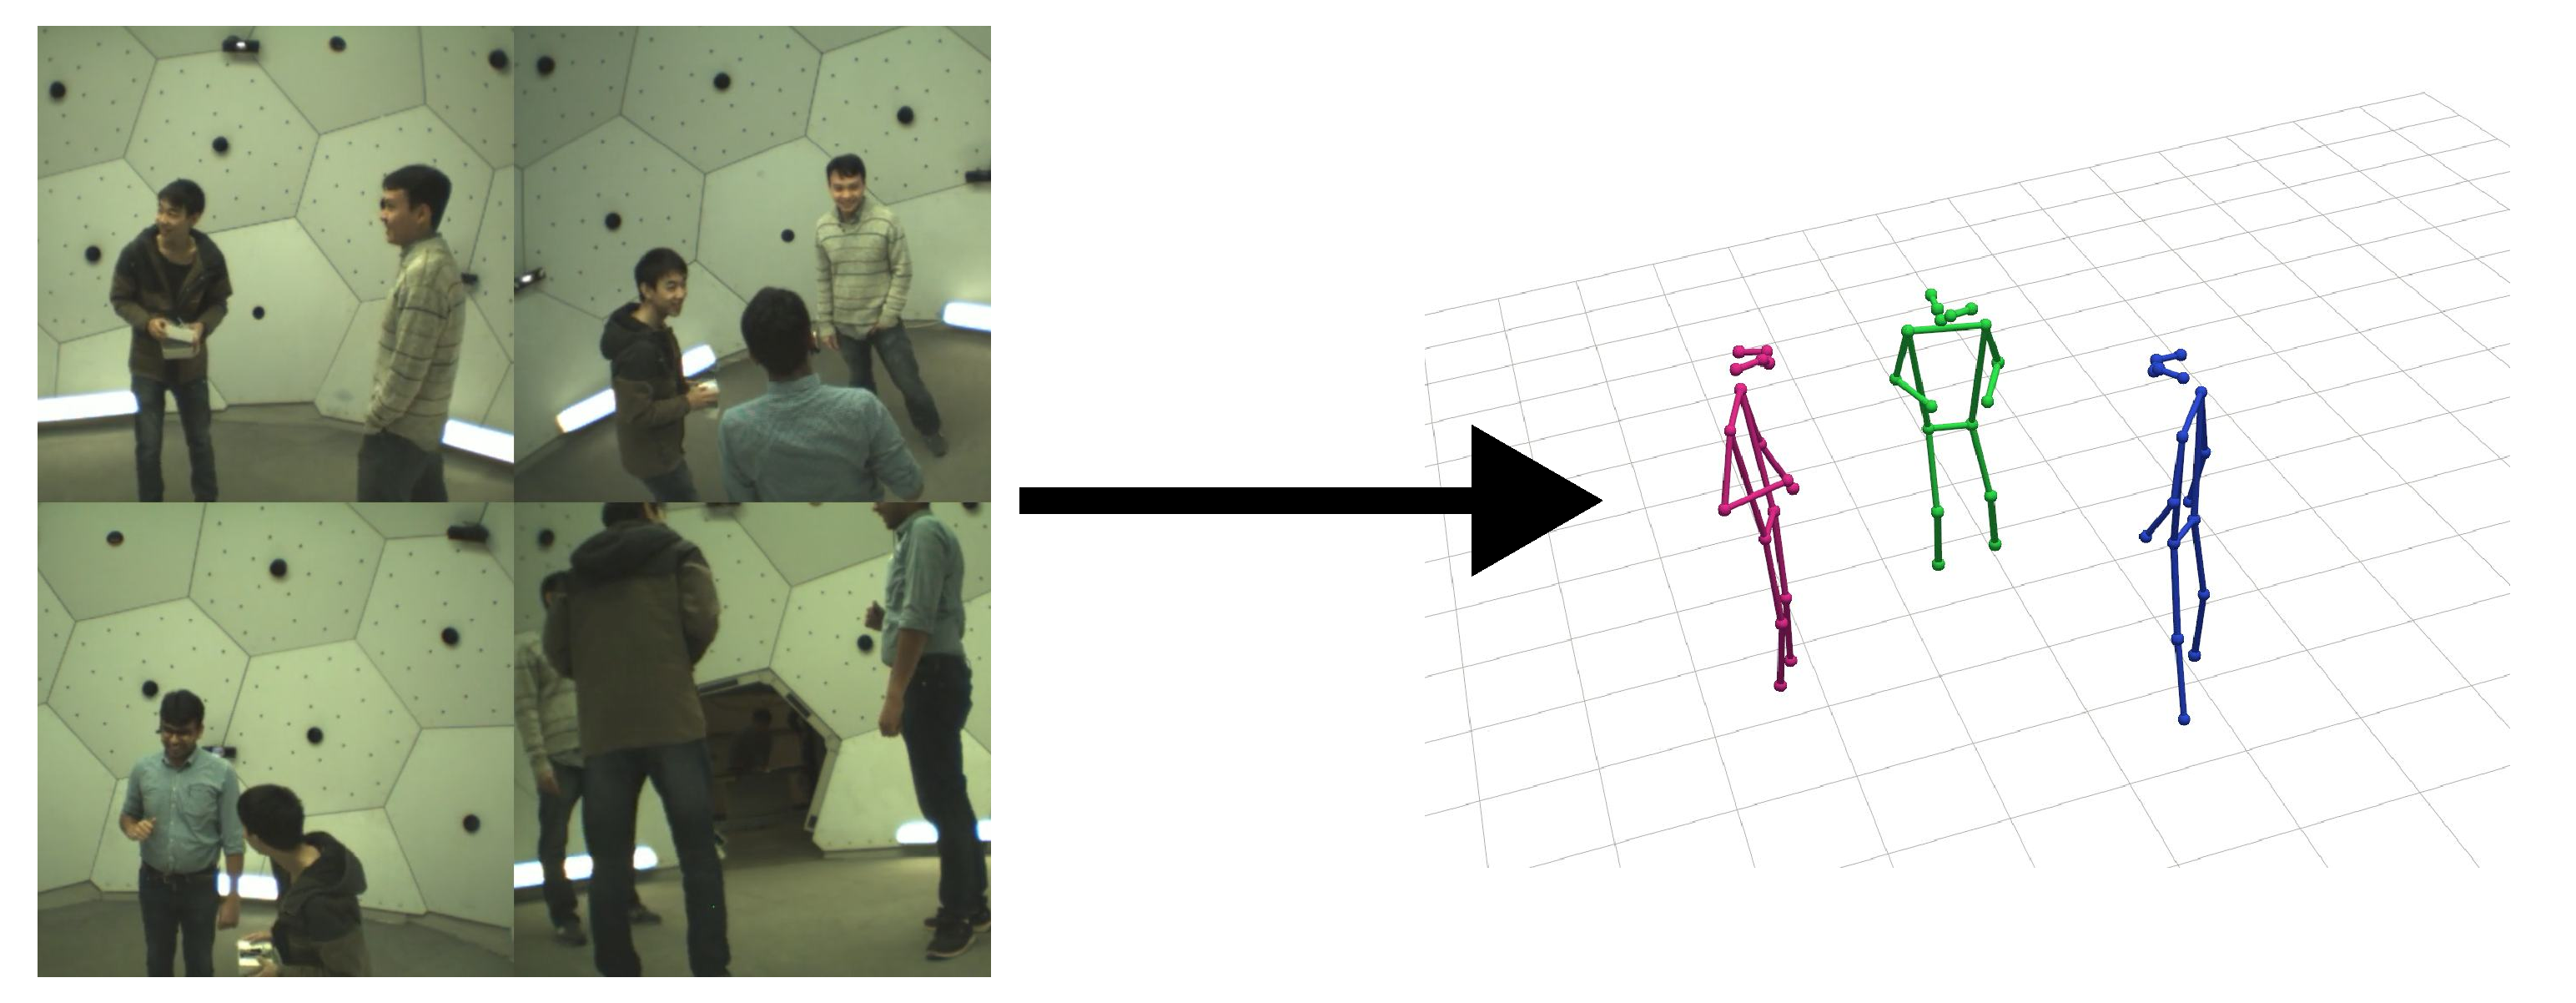
\includegraphics[width=0.9\linewidth]{figures/introduction.pdf}
    \end{figure}
  \end{items}
\end{frame}

\begin{frame}
\frametitle{What to do next?}
  \begin{items}
    \begin{oitem}{\litem}
      Summary: \\
      \sitem {\footnotesize Joint spatiotemporal modeling (ConvGRU) offers the best accuracy.} \\
      \sitem {\footnotesize However, stacked CNN may be preferred, as lower-resource alternative for real-time use.}
    \end{oitem}
    \begin{oitem}{\litem}
      Limitations: \\
      \sitem {\footnotesize Blurry predictions due to loss function.} \\
      \sitem {\footnotesize High computational cost for recurrent models.}
    \end{oitem}
    \begin{oitem}{\litem}
      Possible Future Improvements: \\
      \sitem {\footnotesize Use SSIM or GAN (Adversarial) loss to sharpen images.} \\
      \sitem {\footnotesize Incorporate raw satellite channels or weather data.}\\
      \sitem {\footnotesize Train natively with autoregressive feedback.} \\
      \sitem {\footnotesize Use more advanced recurrent units, e.g., TrajGRU or LSTA.}
    \end{oitem}
  \end{items}
\end{frame}

{
\setbeamercolor{background canvas}{bg=black}
\begin{frame}[plain]{}
\end{frame}
}

\end{document}
